\documentclass[12pt,letterpaper]{exam}
\usepackage[lmargin=1in,rmargin=1in,tmargin=1in,bmargin=1in]{geometry}
\usepackage{../style/exams}

% -------------------
% Course & Exam Information
% -------------------
\newcommand{\course}{MAT 100: Exam 2}
\newcommand{\term}{Fall -- 2022}
\newcommand{\examdate}{11/14/2022}
\newcommand{\timelimit}{85 Minutes}

\setbool{hideans}{false} % Student: True; Instructor: False

% -------------------
% Content
% -------------------
\begin{document}

\examtitle
\instructions{Write your name on the appropriate line on the exam cover sheet. This exam contains \numpages\ pages (including this cover page) and \numquestions\ questions. Check that you have every page of the exam. Answer the questions in the spaces provided on the question sheets. Be sure to answer every part of each question and show all your work.} 
\scores
%\bottomline
\newpage

% ---------
% Questions
% ---------
\begin{questions}

% Question 1
\newpage
\question[10] Suppose that the milage of a car, $M$, after $t$~years is modeled by $M(t)= 8500t + 48000$. 
	\begin{enumerate}[(a)]
	\item Find the number of miles on the car after 4~years.
	\item How long until the car's milage is 100,000~miles?
	\end{enumerate} \pspace

{\itshape
\sol 
\begin{enumerate}[(a)]
\item The number of miles on the car after $t= 4$ years is $M(4)$. We have\dots
	\[
	M(4)= 8500(4) + 48000= 34000 + 48000= 82000
	\]
Therefore, after 4~years, the car has 82,000~miles on it. \pspace

\item If the millage on the car is 100,000~miles, then we have $M(t)= 100000$. But then\dots
	\[
	\begin{aligned}
	M(t)&= 100000 \\[0.3cm]
	8500t + 48000&= 100000 \\[0.3cm]
	8500t&= 520000 \\[0.3cm]
	t&\approx 6.12
	\end{aligned}
	\]
Therefore, the car will have 100,000~miles on it after 6.12~years, i.e. 6~years and 43.8~days.  
\end{enumerate}
}



% Question 2
\newpage
\question[10] Suppose that a worker at a local warehouse is paid an hourly wage of \$20/hour. Explain why the worker's net salary is a linear function. \pspace

{\itshape
Because the worker's hourly wage is fixed, their net salary has a constant rate of change. But then their net salary must be a linear function of the number of hours that they work. 
}



% Question 3
\newpage
\question[10] An oil company is selling off oil in one of their reserves. The amount of oil in the tank in gallons, $O$, after $d$ days is given by $O(d)= 180000 - 19000d$.
	\begin{enumerate}[(a)]
	\item Find and interpret the slope of $O(d)$ in the context of the problem. 
	\item Find and interpret the $y$-intercept of $O(d)$ in the context of the problem. 
	\end{enumerate} \pspace

{\itshape First, observe that $O(d)= 180000 - 19000d$ has the form $y= mx + b$ with $m= -19000$ and $b= 180000$. 
\begin{enumerate}[(a)]
\item The slope of $O(d)$ is $m= -19000$. Thinking of $m$ as $m= \frac{\Delta O}{\Delta d}= \frac{-19000}{1}$, we can see that for each additional day, the amount of oil in the tank decreases by $-19000$; that is, the oil company sells 19,000 gallons of oil in the tank each day. \pspace

\item The $y$-intercept of $O(d)$ is $b= 180000$. This is the amount of oil in the tank at $d= 0$. Therefore, at the start of the sale, there was 180,000~gallons of oil in the tank. 
\end{enumerate}
}



% Question 4
\newpage
\question[10] If the CPI was \$284.581 last year and this year it is \$301.779, find the inflation rate from last year to this year. \pspace

{\itshape
We have\dots \par\vspace{0.1cm}
	\[
	\dfrac{\$301.779}{\$284.581} \approx 1.06043= 1 + 0.06043
	\] \pspace
Therefore, the inflation rate was 6.043\%. 
}



% Question 5
\newpage
\question[10] Suppose you make \$72,000 in a year and take a standard deductible of \$13,200. Find your federal income tax. \par
	\begin{table}[!ht]
	\centering
	\begin{tabular}{|l|l|} \hline
	Tax Rate & Taxable Income \\ \hline \hline
	10\% & Up to \$10,275 \\ \hline
	12\% & \$10,276 -- \$41,775 \\ \hline
	22\% & \$41,776 -- \$89,075 \\ \hline
	24\% & \$89,076 -- \$170,050 \\ \hline
	32\% & \$170,051 -- \$215,950 \\ \hline
	35\% & \$215,951 -- \$539,900 \\ \hline
	37\% & $\geq$ \$539,901 \\ \hline
	\end{tabular}
	\end{table} \pspace

{\itshape 
Your taxable income is $\$72,000 - \$13,200= \$58,800$. Therefore, your federal income tax is\dots
	\[
	\begin{aligned}
	\text{Income Tax}&= 0.10(\$10275 - \$0) + 0.12(\$41775 - \$10275) + 0.22(\$58800 - \$41775) \\[0.3cm]
	&= 0.10(\$10275) + 0.12(\$31500) + 0.22(\$17025) \\[0.3cm]
	&= \$1027.50 + \$3780 + \$3745.50 \\[0.3cm]
	&= \$8553.00
	\end{aligned}
	\]
Therefore, you pay \$8,553.00 in federal income taxes. 
}



% Question 6
\newpage
\question[10] If you placed \$500 into an account which earns 1.2\% annual interest, compounded semiannually, how long until there is \$600 in the account? \pspace

{\itshape
If $P$~dollars is gaining interest at an annual interest rate $r$ each year, compounded $k$ timers per year, then the amount of time this amount $P$ takes to reach $F$ dollars is $t= \dfrac{\ln(F/P)}{k \ln(1 + r/k)}$. We have $P= \$500$, $r= 0.012$, and $F= \$600$. Because the interest is compounded semiannually, the interest is compounded twice per year, i.e. $k= 2$. Therefore, we have\dots
	\[
	t= \dfrac{\ln(F/P)}{k \ln(1 + r/k)}= \dfrac{\ln(\$600/\$500)}{2 \ln \left(1 + \frac{0.012}{2} \right)}= \dfrac{\ln(1.2)}{2 \ln(1.006)}= \dfrac{\ln(1.2)}{2(0.00598207)}= \dfrac{0.182322}{0.0119641} \approx 15.24
	\]
Therefore, the account will have \$600 after. 15.24~years, i.e. 15~years, 3~months, and 3.5 days. 
}



% Question 7
\newpage
\question[10] Suppose that you take out a loan for \$13,000 at 6.5\% annual interest, compounded monthly. How much do you owe on the loan after 3~years? \pspace

{\itshape
We know that $P$~dollars gaining interest at an annual interest rate $r$ each year, compounded $k$ times per year for $t$~years is given by $P \left(1 + \dfrac{r}{k} \right)^{kt}$. We have $P= \$13000$, $r= 0.065$, and $t= 3$~years. Because the interest is compounded monthly, the interest is compounded 12 times per year, i.e. $k= 12$. But then we have\dots
	\[
	\begin{aligned}
	F&= P \left(1 + \dfrac{r}{k} \right)^{kt} \\[0.3cm]
	&= \$13000 \left(1 + \dfrac{0.065}{12} \right)^{12 \cdot 3} \\[0.3cm]
	&= \$13000 (1.0054167)^{36} \\[0.3cm]
	&= \$13000 (1.214673) \\[0.3cm]
	&\approx \$15790.75
	\end{aligned}
	\]
Therefore, you owe \$15,790.75 at the end of the 3~years. 
}



% Question 8
\newpage
\question[10] If you invest \$5,400 in an account which earns 2.3\% annual interest, compounded quarterly, how much interest has been earned from this investment after 6~years? \pspace

{\itshape
We know that $P$~dollars gaining interest at an annual interest rate $r$ each year, compounded $k$ times per year for $t$~years is given by $P \left(1 + \dfrac{r}{k} \right)^{kt}$. We have $P= \$5400$, $r= 0.023$, and $t= 6$~years. Because the interest is compounded quarterly, the interest is compounded 4 times per year, i.e. $k= 4$. But then we have\dots
	\[
	\begin{aligned}
	F&= P \left(1 + \dfrac{r}{k} \right)^{kt} \\[0.3cm]
	&= \$5400 \left(1 + \dfrac{0.023}{4} \right)^{4 \cdot 6} \\[0.3cm]
	&= \$5400 (1.00575)^{24} \\[0.3cm]
	&= \$5400 (1.14752192) \\[0.3cm]
	&\approx \$6196.62
	\end{aligned}
	\]
Any additional money above the initial \$5,400 investment must have come from interest. Therefore, the account earned $\$6196.62 - \$5400= \$796.62$ in interest. 
}



% Question 9
\newpage
\question[10] Researchers at a think tank work in a variety of fields and have a wide range of ages. Below is a summary of the workers at the facility. \par
	\begin{table}[!ht]
	\centering
	\begin{tabular}{|c||c|c|c|c||c|} \hline
	& Biology & Chemistry & Physics & Computer Science & Total \\ \hline
	18 -- 30 & 26 & 25 & 18 & 10 & 79 \\ \hline
	30 -- 40 & 21 & 19 & 13 & 17 & 70 \\ \hline 
	40 -- 60 & 14 & 18 & 19 & 28 & 79 \\ \hline
	60+ & 13 & 19 & 22 & 22 & 76 \\ \hline \hline
	Total & 74 & 81 & 72 & 77 & 304 \\ \hline
	\end{tabular}
	\end{table} \par

\begin{enumerate}[(a)]
\item Find the probability that a randomly selected worker is 30--40 or researches Physics.
\item Find the probability that a randomly selected worker is over 60 and researchers Biology.
\item Find the probability that Computer Science researcher is 18--30. 
\end{enumerate} \pspace

\sol 
\begin{enumerate}[(a)]
\item 
	\[
	P(\text{30--40 or Physics})= \dfrac{70 + 72 - 13}{304}= \dfrac{129}{304} \approx 0.4243
	\] \pspace
	
\item 
	\[
	P(\text{Over 60 and Biology})= \dfrac{13}{304} \approx 0.0428
	\] \pspace

\item 
	\[
	P(\text{18--30} \;|\; \text{Computer Science})= \dfrac{10}{77} \approx 0.1299
	\]
\end{enumerate}



% Question 10
\newpage
\question[10] Researchers are investigating people's movie preferences. Below is a summary of their data broken down by gender. \par
	\begin{table}[!ht]
	\centering
	\begin{tabular}{|l||c|c|c|c||c|} \hline
	& Action & Horror & Comedy & Drama & Total \\ \hline
	Male & 60 & 45 & 70 & 53 & 228 \\ \hline
	Female & 51 & 38 & 65 & 67 & 221 \\ \hline 
	Unspecified & 40 & 30 & 20 & 15 & 105 \\ \hline \hline
	Total & 151 & 113 & 155 & 135 & 554 \\ \hline
	\end{tabular}
	\end{table} \par

\begin{enumerate}[(a)]
\item Find the percentage of people that were female or preferred horror. 
\item Find the percentage of people that were male and preferred drama.
\item Assuming a person preferred action, what was the probability that their gender was unspecified? 
\end{enumerate} \pspace

\sol 
\begin{enumerate}[(a)]
\item 
	\[
	P(\text{female or horror})= \dfrac{221 + 113 - 38}{554}= \dfrac{296}{554} \approx 0.5343
	\] \pspace

\item 
	\[
	P(\text{male and drama})= \dfrac{53}{554} \approx 0.0957
	\] \pspace

\item 
	\[
	P(\text{unspecified} \;|\; \text{action})= \dfrac{40}{151} \approx 0.2649
	\]
\end{enumerate}



% Question 11
\newpage
\question[10] At a local college with 1,540 students, 431 students have a minor in a STEM field, 687 students have a minor in the Humanities, and 84 students have a minor in both. Complete the Venn diagram below and find the percentage of students that do not have a minor in STEM nor the Humanities. 
	\[
	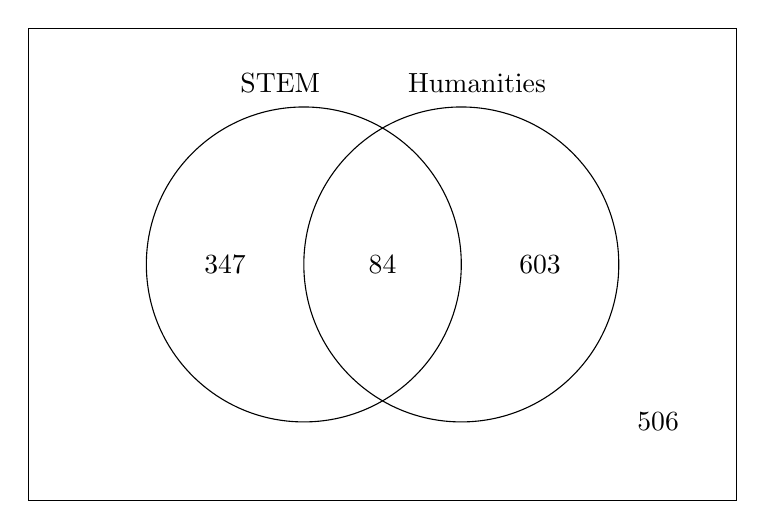
\begin{tikzpicture}
	\draw (0,0) rectangle (9,6);
	\draw (3.5,3) circle (2);
	\draw (5.5,3) circle (2);
	
	\node at (3.2,5.3) {STEM};
	\node at (5.7,5.3) {Humanities}; 
	
	\node at (2.5,3) {347};
	\node at (4.5,3) {84};
	\node at (6.5,3) {603};
	\node at (8,1) {506};
	\end{tikzpicture}
	\] 
	
	\[
	P(\text{not STEM nor Humanities})= \dfrac{506}{1540} \approx 0.3286
	\] \pspace
Therefore, approximately 32.86\% of students do not have a minor in STEM nor the Humanities. 



% Question 12
\newpage
\question[10] Suppose that if a student studies for an exam, there is an 85\% chance that they pass the exam. If a student does not study for an exam, there is a 80\% chance that they fail the exam. A school estimates that 70\% of their students study for their exams. Complete the tree diagram below and find the percentage of students at this school that fail their exam. 
	\[
	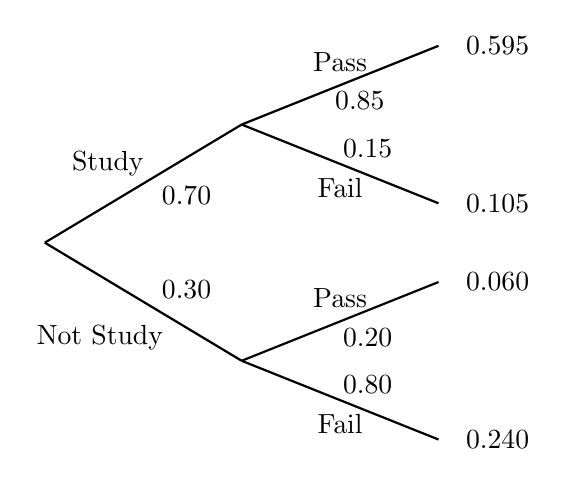
\begin{tikzpicture}[scale= 1.0]
	\def\FirstUpLabel{Study}
	\def\FirstDownLabel{Not Study}
	\def\SecondUpLabel{Pass}
	\def\SecondDownLabel{Fail}
	\def\Up{$0.70$}
	\def\Down{$0.30$}
	\def\UpUp{$0.85$}
	\def\UpDown{$0.15$}
	\def\DownUp{$0.20$}
	\def\DownDown{$0.80$}
	\def\first{$0.595$}
	\def\second{$0.105$}
	\def\third{$0.060$}
	\def\fourth{$0.240$}
		
	\node at (0.8,1) {\FirstUpLabel};	
	\node at (0.7,-1.2) {\FirstDownLabel};	
	\node at (1.8,0.6) {\Up};
	\node at (1.8,-0.6) {\Down};
	\draw[thick] (0,0) -- (2.5,1.5);
	\draw[thick] (0,0) -- (2.5,-1.5);
		
	\node at (3.75,2.3) {\SecondUpLabel};
	\node at (3.75,0.7) {\SecondDownLabel};
	\node at (4,1.8) {\UpUp};
	\node at (4.1,1.2) {\UpDown};
	\node at (5.75,2.5) {\first};
	\node at (5.75,0.5) {\second};
	\draw[thick] (2.5,1.5) -- (5,2.5);
	\draw[thick] (2.5,1.5) -- (5,0.5);

	\node at (3.75,-0.7) {\SecondUpLabel};
	\node at (3.75,-2.3) {\SecondDownLabel};
	\node at (4.1,-1.2) {\DownUp};
	\node at (4.1,-1.8) {\DownDown};
	\node at (5.75,-0.5) {\third};	
	\node at (5.75,-2.5) {\fourth};	
	\draw[thick] (2.5,-1.5) -- (5,-0.5);
	\draw[thick] (2.5,-1.5) -- (5,-2.5);
	\end{tikzpicture}
	\] \pspace
	
	\[
	P(\text{fail})= 0.105 + 0.240= 0.345
	\] \pspace

Therefore, 34.5\% of students at the school fail their exam. 



% Question 13
\newpage
\question[10] The probability of a car over 10~years old having a critical issue is 45\%. Researchers estimate that 13\% of cars are Ford brand cars. The same researchers then estimate that $0.45 \cdot 0.13= 0.0585 \squiggle 5.85\%$ of cars that are over 10~years old having a critical issue are Ford brand. Explain what is wrong with the researchers mathematical calculation. \pspace

{\itshape
If $A$ and $B$ are events, we know that $P(A \text{ and } B)= P(A) \cdot P(B)$ only if $A$ and $B$ are independent. Generally, we have $P(A \text{ and } B)= P(A) \cdot P(B \;|\; A)= P(B) \cdot P(A \;|\; B)$. Here $A$ can be the event that a car has a critical issue and $B$ is the event that a car is a Ford. Because one does not know if these events are independent, i.e. that Ford brand cars have more/less critical issues as they age, we cannot be sure that $P(A \text{ and } B)= 0.45 \cdot 0.13= 0.0585$. 
}


\end{questions}
\end{document}